\chapter{Vorlesung 1: Themen der Stringtheorie}

\lectureoverview{Die Herausforderung des Reduktionismus wird durch die Bosonisierung in \(1+1\) Dimensionen, die elektrische--magnetische Dualität, D-Branen, Übergänge bei starker Kopplung, emergente Geometrie und die kombinatorische Landschaft der Stringvakuua zugespitzt. Dasselbe physikalische System kann sehr unterschiedliche elementare Beschreibungen zulassen; welche davon einfach erscheint, hängt von der Kopplung und der Geometrie ab.}

\section{Reduktionismus, Komplexität und die Frage nach der Einfachheit}

Susskind beginnt mit einem bewusst vertrauten philosophischen Slogan: Große Dinge bestehen aus kleinen Dingen, und kleine Dinge aus noch kleineren. Dann fügt er die anspruchsvollere Fassung desselben Gedankens hinzu, auf die es für die fundamentale Physik wirklich ankommt: Wenn man zu tieferen Schichten vordringt, sollten die Objekte nicht nur kleiner, sondern auch einfacher werden. Sein Bild: Häuser bestehen aus Ziegeln, und niemand verwechselt ein Haus mit einem Ziegel. Der Ziegel ist kleiner, aber auch einfacher.

Als ersten Schritt konfrontiert die Vorlesung diese Erwartung mit dem tatsächlichen Stand der Teilchenphysik. Würde der Reduktionismus in diesem starken Sinn zu wachsender Einfachheit führen, könnte man erwarten, dass die heutige Elementarteilchenphysik überschaubar wäre. Stattdessen betont Susskind, dass die Bestandsaufnahme schon vor Einbeziehung der Quantengravitation unübersichtlich aussieht. Die Zahlen in der Vorlesung sind grobe Schätzungen, doch gerade das gehört zum Argument:
\begin{equation}
\begin{aligned}
N_{\mathrm{species}}&\sim 75,\\
N_{\mathrm{independent}}&\sim 10\text{--}20,\\
N_{\mathrm{parameters}}&\sim 20.
\end{aligned}
\end{equation}
Damit ist die Geschichte noch nicht zu Ende. Das Standardmodell enthält keine Gravitation, erklärt die Dunkle Materie nicht, liefert nicht die für die Inflation erforderliche zusätzliche Struktur und weist ein gravierendes Feinabstimmungsproblem auf. Die üblichen Lösungsansätze erhöhen die Zahl nur weiter. Als Beispiel nennt die Vorlesung die Supersymmetrie. Zur Zeit der Vorlesung hofften viele Physiker, der Large Hadron Collider werde Superpartner nachweisen. Susskind betont, dass die entsprechende Erweiterung die Bestandsaufnahme um mehr als hundert zusätzliche Parameter vergrößern würde, statt sie unmittelbar zu vereinfachen. Seine schematische Aussage lautet:
\begin{equation}
N_{\mathrm{parameters}}^{\mathrm{extended}} \sim 200.
\end{equation}
Diese Zahlen sind bewusst grob und an den damaligen Stand gebunden. Sie veranschaulichen das Argument, dass eine tiefere Beschreibung hinsichtlich ihres Teilchenbestands und ihrer gemessenen Konstanten nicht unbedingt einfacher aussehen muss.

Diese quantitative Kritik ist noch nicht Susskinds Hauptthese, sondern deren Vorbereitung. Die weitergehende Behauptung, die den Rest der Vorlesung bestimmt, lautet, dass die moderne Quantenfeldtheorie und die Stringtheorie keine eindeutige, von der Kopplung unabhängige Unterscheidung zwischen Ziegeln und Häusern nahelegen. Die folgenden Beispiele sollen zeigen, dass die Bedeutung von ``elementar'' davon abhängen kann, welche Variablen sich effizient verwenden lassen.

\section{Bosonisierung: Ein erstes Aufbrechen fester Fundamentalität}

Susskinds erstes theoretisches Beispiel stammt aus einer Quantenfeldtheorie in \(1+1\) Dimensionen: einer Raum- und einer Zeitdimension. Gleich zu Beginn kündigt er an, dass er die Äquivalenz nicht im Einzelnen herleiten wird; es gehe nicht um den formalen Beweis, sondern um die begriffliche Einsicht.

Ausgangspunkt ist eine Feldtheorie von Fermionen. Das Fermionfeld wird mit \(\psi\) bezeichnet. Zwei nahe beieinanderliegende Fermionen können einen bosonischen Verbund bilden; das zugehörige Bosonenfeld wird mit \(\phi\) bezeichnet. Auf den ersten Blick scheint die Hierarchie klar: \(\psi\) ist fundamental, während \(\phi\) eine zusammengesetzte oder effektive Variable ist. In der Vorlesung wird das Boson genau so eingeführt: als Feld, das gebundene Fermionenpaare erzeugt.

Es stellte sich jedoch heraus, dass sich dieselbe Theorie mit umgekehrtem Ausgangspunkt formulieren lässt. Man kann mit dem Bosonenfeld \(\phi\) beginnen; dann erscheint das Fermion nicht mehr als punktförmiger Bestandteil. Stattdessen tritt es als Knick des Bosonenfeldes auf, als ausgedehnte Konfiguration, in der \(\phi\) glatt zwischen zwei asymptotischen Werten interpoliert. Der minimale mathematische Inhalt der Vorlesung ist diese asymptotische Struktur:
\begin{equation}
\phi(x\to -\infty)=\phi_-,
\qquad
\phi(x\to +\infty)=\phi_+.
\end{equation}
Eine zweckmäßige schematische Darstellung ist
\begin{equation}
\phi(x)\approx \frac{\phi_++\phi_-}{2}
+
\frac{\phi_+-\phi_-}{2}\tanh\!\left(\frac{x}{\ell}\right),
\end{equation}
Dabei bezeichnet \(\ell\) die Breite des Übergangsbereichs.

\editorialnote{Das Hyperbeltangens-Profil ist eine übliche glatte Darstellung des in der Vorlesung skizzierten Knicks, keine dort hergeleitete Formel. Die genaue Bosonisierungszuordnung hängt vom Modell ab; entscheidend ist der begriffliche Austausch zwischen einer fermionischen Anregung und einem topologischen Soliton eines Bosonenfeldes.}

Die Gürtelanalogie der Vorlesung ist anschaulich genug, um sie beizubehalten. Ein flach liegender, unverdrehter Gürtel entspricht einer Konfiguration ohne Knick. Dreht man ein Ende um \(2\pi\), hat der Gürtel weit entfernt wieder dieselbe lokale Ausrichtung, muss dazwischen aber einen ausgedehnten verdrehten Bereich durchlaufen. Dieser verdrehte Bereich ist der Knick. In der bosonischen Beschreibung wird das Fermion genau durch ein solches ausgedehntes Objekt dargestellt.

Mit der Einführung einer Kopplung wird der Punkt deutlicher. Susskind bezeichnet sie in diesem Beispiel mit \(G\). Die Aussage lautet nicht bloß, dass die beiden Beschreibungen irgendwie zusammenhängen, sondern dass ihre Effizienz vom Parameterbereich abhängt:
\begin{align}
G \ll 1
&\Rightarrow
\ell\text{ small, tight kink; }\psi\text{ efficient},\\
G \gg 1
&\Rightarrow
\ell\text{ large, broad kink; }\phi\text{ efficient}.
\end{align}
Für kleine Werte von \(G\) ist der Knick schmal und das Fermion erscheint als einfaches Objekt. Mit zunehmendem \(G\) wird der Knick breiter und das Fermion weniger punktförmig. Dann sind die bosonischen Variablen die sparsamere Beschreibung.

\paragraph{Schematischer Ablauf.}
\begin{enumerate}
\item Ausgangspunkt ist eine fermionische Theorie, beschrieben durch \(\psi\).
\item Bosonische Verbünde identifizieren, beschrieben durch \(\phi\).
\item Dieselbe Theorie vollständig in Termen von \(\phi\) umformulieren.
\item In der bosonischen Beschreibung tritt das Fermion als Knick der Breite \(\ell\) wieder auf.
\item Für \(G\ll 1\) ist \(\ell\) klein und die fermionische Beschreibung am einfachsten.
\item Bei größerem \(G\) wächst \(\ell\), und die bosonische Beschreibung wird am einfachsten.
\end{enumerate}

Dies ist das erste ausdrückliche Gegenbeispiel zum festen Bild von ``Häusern und Ziegeln''. Die Pointe der Vorlesung ist nicht bloß, dass zusammengesetzte Objekte existieren, sondern dass sich je nach Kopplung ändern kann, welche Variable als elementar gilt.

\section{Elektrische Ladung, magnetische Monopole und schwache gegenüber starker Kopplung}

Als Nächstes fragt Susskind, ob sich eine ähnliche Geschichte auch in der vertrauteren Teilchenphysik findet. Sein Beispiel ist der Gegensatz zwischen elektrischer Ladung und magnetischem Monopol. Ein gewöhnliches geladenes Teilchen wie das Elektron ist in dieser Sprache ein elektrischer Monopol: eine lokalisierte Quelle eines elektrischen Feldes. Der magnetische Monopol wird anhand eines Stabmagneten eingeführt. Könnte man das Ende eines Stabmagneten irgendwie isolieren, ohne den unsichtbaren verbindenden Stab, sähen die Feldlinien genauso aus wie die eines elektrischen geladenen Teilchens, wären aber magnetischer statt elektrischer Natur.

Der maßgebliche Kontrollparameter ist die Feinstrukturkonstante \(\alpha\). In der Vorlesung behandelt Susskind sie heuristisch als Quadrat der elektrischen Ladung:
\begin{equation}
\alpha \sim e^2.
\end{equation}
Außerdem gibt er eine grobe operationale Deutung: Sie misst, wie leicht ein Elektron Strahlung emittiert. Die Stärke fasst er so zusammen, dass ein beschleunigtes Elektron in dem hier gemeinten Sinn Photonen in einer Größenordnung von ``\(1/100\)'' abstrahlt. In der groben numerischen Sprache der Vorlesung:
\begin{equation}
\alpha \approx 10^{-2}.
\end{equation}
Das ist nicht als präzise Konvention gedacht, sondern als didaktische Möglichkeit auszudrücken, dass die elektrische Ladung schwach ist.

\editorialnote{Der Zusammenhang zwischen schwacher--starker Kopplung hat einen präzisen Vorläufer in der Dirac-Quantisierung. In einer verbreiteten Konvention erfüllen elektrische und magnetische Ladungen die Beziehung \(e g_m=2\pi n\). Eine schwache elektrische Kopplung entspricht damit einer starken magnetischen, auch wenn genaue numerische Faktoren und geschützte Massenbeziehungen von der Theorie abhängen.}

Für \(\alpha\ll 1\) ist das Elektron das einfache Objekt. Sein elektrisches Feld ist schwach, seine Vakuumpolarisationswolke dünn, und es erscheint nahezu punktförmig. Beim magnetischen Monopol ist es umgekehrt: Sein Feld ist enorm, seine Umgebung stark verzerrt, und er ist ausgedehnt, kompliziert und schwer. Susskind fasst die Lage genau in diesem Stil schwacher--starker Kopplung zusammen:
\begin{equation}
\begin{aligned}
\alpha \ll 1
&\Rightarrow \text{simple electron;}\\
&\phantom{\Rightarrow{}}\text{heavy, extended monopole},\\
\alpha \gg 1
&\Rightarrow \text{simple monopole;}\\
&\phantom{\Rightarrow{}}\text{heavy, structured electron}.
\end{aligned}
\end{equation}
Die Vorlesung leitet keine Massenformel für den Monopol her; das ist auch nicht nötig. Entscheidend ist die qualitative Aussage. Mit zunehmendem \(\alpha\) wird das Feld des Elektrons stärker und seine Struktur wächst, während der Monopol schrumpft und leichter wird. Weit oberhalb der Einheit kehrt sich die zweckmäßigste Beschreibung um: Der Monopol ist einfach und das Elektron kompliziert.

Das ist die feldtheoretische Fassung der früheren Einsicht aus der Bosonisierung. Die Unterscheidung zwischen fundamental und zusammengesetzt ist nicht absolut, sondern hängt von der Kopplung ab.

\begin{classroomqa}\audiencequestion{Wenn der Reduktionismus kein verlässlicher Wegweiser ist, warum verlassen sich Physiker dann auf die Infinitesimalrechnung, die ein System scheinbar in beliebig kleine Teile zerlegt? \lecturetimestamp{00:21:21}}\lecturerresponse{Die Infinitesimalrechnung beschreibt glatte Veränderungen; sie legt nicht fest, welche Objekte in einer Theorie fundamental sind. Quantenfelder fluktuieren auf jeder Längenskala. So entsteht eine endlose Hierarchie statt einer letzten glatten Schicht, auf der sich ein für alle Mal entscheiden ließe, was elementar ist.}\end{classroomqa}

Die Diskussion geht mit dem Vorschlag weiter, die Hierarchie ähnele einem Fraktal. Susskind stimmt der Analogie zu und präzisiert sie dann: Quantenfelder fluktuieren auf jeder Skala und sind daher im klassischen Sinn niemals glatt. Diese übermäßigen Schwankungen tragen zur mathematischen Schwierigkeit der Quantenfeldtheorie bei; die gewöhnliche Infinitesimalrechnung muss mit renormierten Größen arbeiten und nicht mit einem naiv glatten mikroskopischen Feld.

\section{Strings, D-Branen und die Rückkehr der Dualität zwischen schwacher--starker Kopplung}

Der nächste Übergang in der Vorlesung ist bewusst naiv. Wenn die Stringtheorie die Theorie der fundamentalen Bausteine sein soll, dann muss die Antwort doch einfach sein: Die Bausteine sind Strings. Susskind spricht diese Erwartung ausdrücklich aus und verwendet dann den nächsten Teil der Vorlesung darauf, sie zu erschüttern.

\subsection{Warum Strings nicht die ganze Geschichte sind}

Die erste Komplikation ist die unvermeidliche Existenz von D-Branen. Eine D\(p\)-Brane ist ein Objekt mit \(p\) Dimensionen, an dem Strings enden können. Der Buchstabe \(D\) geht auf Dirichlet-Randbedingungen zurück, doch der Name ist weit weniger wichtig als die Funktion: Diese Objekte gehören zur Theorie und lassen sich nicht weglassen. Sie sind keine optionalen Verzierungen.

Die einfachsten Beispiele sind:
\begin{itemize}
\item eine D0-Brane, die punktförmig ist,
\item eine D1-Brane oder ein D-String, der stringartig ist,
\item ein F-String, der gewöhnliche fundamentale String.
\end{itemize}
Eine D0-Brane ist ein schwerer, punktförmiger Ort, an dem beliebig viele F-Strings enden können. Eine D1-Brane ist ein schweres, kabelartiges Objekt, das deutlich dicker ist und mehr Masse pro Längeneinheit besitzt als ein F-String, aber ebenfalls Endpunkte für F-Strings bietet. Bei schwacher Kopplung stellt die Vorlesung diese Objekte nicht als gleichwertige elementare Alternativen dar. D-Branen werden als schwere, strukturierte, zusammengesetzt wirkende Objekte eingeführt, die uns die Theorie dennoch aufzwingt.

\editorialnote{Die in diesem Teil der Vorlesung verwendete Theorie mit ungeraden Branen ist die Stringtheorie vom Typ IIB. Ihre stabilen D-Branen haben ungerade räumliche Dimensionen, darunter D1- und D3-Branen. Susskind schiebt diese Bezeichnungen auf, weil zunächst das Dualitätsmuster und nicht die Taxonomie im Mittelpunkt steht.}

\paragraph{Notation.}
Susskind verwendet \(G\) und \(g\) in verschiedenen Teilen der Vorlesung nicht ganz einheitlich. Hier steht \(G\) für das Bosonisierungsbeispiel, während \(g\) die Stringkopplung bezeichnet.

Die Stringkopplung \(g\) wird operational definiert, nicht axiomatisch. Sie ist der Parameter, der die Wahrscheinlichkeit dafür angibt, dass ein fluktuierender String aufspaltet und Tochterstrings bildet. Deshalb vergleicht Susskind ihre Rolle unmittelbar mit der von \(\alpha\) in der Quantenelektrodynamik. Außerdem hält die Vorlesung kurz fest, dass die Spannung der Energie pro Längeneinheit entspricht:
\begin{equation}
T=\frac{E}{L}=\frac{M}{L}.
\end{equation}

Für einen F-String und einen D-String machen die üblichen Spannungsformeln den Vergleich zwischen schwacher--starker Kopplung ausdrücklich:
\begin{equation}
T_{\mathrm{F1}}=\frac{1}{2\pi\alpha'},
\qquad
T_{\mathrm{D1}}=\frac{1}{2\pi\alpha' g_s},
\qquad
\frac{T_{\mathrm{D1}}}{T_{\mathrm{F1}}}=\frac{1}{g_s}.
\end{equation}
\editorialnote{Diese Spannungsformeln liefern die übliche Normierung für den qualitativen Vergleich von Kabel und Faden in der Vorlesung. Sie wurden redaktionell ergänzt; in der Vorlesung wird nur die Skalierung mit der Kopplung verwendet.}

\subsection{F-Strings und D-Strings}

Das Muster schwacher--starker Kopplung wiederholt sich nun in der Sprache der Stringtheorie. Bei kleiner Kopplung ist der F-String leicht und dünn und entspricht weitgehend dem ursprünglichen anschaulichen Bild eines fundamentalen Objekts. Der D-String ist dick, schwer und voller F-String-Struktur. Mit wachsender Kopplung spaltet sich der F-String leichter auf; die Wolke aus Tochterstrings um ihn herum wird dichter, und er wird schwerer und komplizierter. Gleichzeitig fällt es dem D-String zunehmend schwer, die nun schweren F-Strings zu emittieren. Seine umgebende Struktur lichtet sich, und er wird leichter und linienartiger. Die Zuordnung schwacher--starker Kopplung in der Vorlesung lautet daher:
\begin{align}
g \ll 1
&\Rightarrow
\begin{gathered}
\text{F-string light and thin;}\\
\text{D-string heavy and structured},
\end{gathered}\\
g \sim 1
&\Rightarrow
\text{F-string and D-string comparable},\\
g \gg 1
&\Rightarrow
\begin{gathered}
\text{D-string light and thin;}\\
\text{F-string heavy and structured}.
\end{gathered}
\end{align}
Susskind merkt an, dass die beiden Beschreibungen bei \(g\sim 1\) nicht mehr klar voneinander zu unterscheiden sind. Jenseits dieses Punktes tauschen sie im Wesentlichen ihre Rollen. Das ist die stringtheoretische Variante des Austauschs zwischen Elektron und Monopol--; sie wird als S-Dualität bezeichnet.

Derselbe Austausch lässt sich auch verfolgen, wenn ein String sich zu einer Schleife schließt. Bei schwacher Kopplung ist eine kleine F-String-Schleife eine leichte, teilchenartige Anregung, während die entsprechende D-String-Schleife schwer und kompliziert ist. Bei starker Kopplung kehren sich ihre Rollen um: Die D-String-Schleife wird zur leichten Beschreibung, und zu den daraus hervorgehenden leichten geschlossenen Stringanregungen gehört das Graviton. Mit diesem Beispiel unterstreicht die Vorlesung, dass sogar die Identität eines vertrauten Teilchens davon abhängen kann, welche Seite der Dualität man verwendet.

Die Vorlesung führt den Gedanken noch einen Schritt weiter. In der idealisierten Theorie ist die Kopplung nicht einfach eine von Hand einstellbare Zahl, sondern verhält sich wie ein Feld. Schematisch:
\begin{equation}
g = g(x).
\end{equation}
Daher können in verschiedenen Raumbereichen unterschiedliche Dualitätsbeschreibungen zweckmäßig sein. In einem Bereich sind F-Strings die leichten Variablen, in einem anderen D-Strings. Dazwischen ist keine der beiden Beschreibungen besonders einfach. Deshalb stellt die Stringtheorie für Susskind das einfache reduktionistische Bild nicht wieder her, sondern verschärft die Mehrdeutigkeit.

\editorialnote{In der perturbativen Stringtheorie wird die lokale Kopplung durch das Dilaton \(g_s(x)=e^{\Phi(x)}\) bestimmt. Die Schreibweise \(g=g(x)\) ist daher mehr als eine Analogie, auch wenn realistische Kompaktifizierungen im Allgemeinen ein Potential erzeugen, das solche Variationen einschränkt.}

\begin{classroomqa}\audiencequestion{Wenn die Kopplung so stark variierte, dass D-Strings in einem anderen Bereich leichter als F-Strings würden, würde sich das auf beobachtbare Spektren auswirken? \lecturetimestamp{00:34:15}}\lecturerresponse{Ja. Das ist einer der Gründe, warum sich das hier betrachtete, exakt symmetrische und mathematisch kontrollierbare Modell nicht unmittelbar mit unserer Welt gleichsetzen lässt. Es geht um das, was konsistente Quantentheorien leisten können, nicht um ein wörtliches Spektrum der Natur.}\end{classroomqa}

\begin{classroomqa}\audiencequestion{Gibt es eine analoge duale Beschreibung für eine D2-Brane? \lecturetimestamp{00:34:39}}\lecturerresponse{Ja, aber es handelt sich nicht um einen weiteren Austausch nach Art der D-Strings. Der Fall geradzahliger Branen führt zu einer Interpretation durch Membranen und zu einer zusätzlichen Raumdimension; das ist die nächste Konstruktion.}\end{classroomqa}

\begin{classroomqa}\audiencequestion{Erklärt eine höhere Aufspaltungswahrscheinlichkeit der Strings die zunehmende innere Komplexität? \lecturetimestamp{00:34:53}}\lecturerresponse{Ja. Um den Mechanismus anschaulich zu machen, kehren wir zur Quantenelektrodynamik zurück: Ein Elektron emittiert Photonen, Photonen fluktuieren zu geladenen Paaren, und diese geladenen Linien strahlen ihrerseits wieder. Bei stärkerer Kopplung wird diese Hierarchie dichter.}\end{classroomqa}

\subsection{Rückkehr zur Quantenelektrodynamik ausgehend von einer Frage}

Ein Student fragt daraufhin, ob die höhere Aufspaltungswahrscheinlichkeit schlicht eine kompliziertere Struktur ``weiter oben'' bedeutet. Susskind antwortet, indem er zur Quantenelektrodynamik zurückkehrt und erneut die Weltlinie des Elektrons zeichnet. Diese Rückkehr ist wichtig: Sie zeigt, dass die Stringgeschichte keine isolierte Kuriosität ist, sondern ein weiteres Beispiel desselben Musters schwacher--starker Kopplung.

\begin{figure}[htbp]\centering
\begin{tikzpicture}[scale=1.0]
\draw[->] (-1.2,0) -- (3.7,0) node[right] {space};
\draw[->] (0,-0.2) -- (0,4.3) node[above] {time};

\draw[line width=0.9pt] (0,0.2) -- (0,4.0);
\node[left] at (0,3.55) {\(e^{-}\)};

\draw[line width=0.8pt] (0,1.0) -- (0.18,1.08) -- (0.36,0.92) -- (0.54,1.10) -- (0.72,0.94) -- (0.90,1.12) -- (1.08,0.96) -- (1.26,1.14);
\draw[line width=0.8pt] (0,2.35) -- (-0.18,2.43) -- (-0.36,2.27) -- (-0.54,2.45) -- (-0.72,2.29) -- (-0.90,2.47);

\draw[line width=0.8pt] (1.26,1.14) -- (1.48,1.42);
\draw[line width=0.8pt] (1.26,1.14) -- (1.04,1.42);
\draw[line width=0.8pt] (1.48,1.42) -- (1.58,2.10);
\draw[line width=0.8pt] (1.04,1.42) -- (0.94,2.10);
\draw[line width=0.8pt] (0.94,2.10) -- (1.58,2.10);

\draw[line width=0.7pt] (1.58,1.78) -- (1.72,1.84) -- (1.86,1.72) -- (2.00,1.86);
\draw[line width=0.7pt] (0.94,1.78) -- (0.80,1.84) -- (0.66,1.72) -- (0.52,1.86);

\node at (2.35,1.95) {\(\gamma\)};
\node at (-1.15,2.75) {\(\gamma\)};
\end{tikzpicture}\caption{Schematische QED-Hierarchie aus der Vorlesung: Ein punktförmiges Elektron emittiert Photonen, Photonen erzeugen Paare, und die geladenen Tochterlinien strahlen erneut. So entsteht Struktur auf immer kleineren Skalen.}\end{figure}

Der Punkt der Vorlesung ist, dass selbst ein punktförmiges Elektron von einer Hierarchie von Prozessen begleitet wird:
\begin{enumerate}
\item Ein Elektron emittiert und absorbiert Photonen.
\item Ein Photon kann ein Elektron--Positron-Paar erzeugen.
\item Die geladenen Tochterlinien können selbst Photonen emittieren.
\item Die Hierarchie setzt sich auf immer kleineren Skalen fort.
\end{enumerate}
Bei schwacher Kopplung ist diese Wolke dünn, sodass das Elektron im Labor nahezu punktförmig erscheint. Bei stärkerer Kopplung wird sie dichter, und das Elektron entwickelt eine innere Struktur. Die Stringgeschichte wird als direkte Analogie dazu vorgestellt.

Dieselbe spätere Diskussion führt auch zu Susskinds heuristischer Energiebilanz. Er betont, dass die relevante Energie nicht bloß die Summe der Beiträge freier Teilchen ist. Auch die Wechselwirkungsenergie muss berücksichtigt werden:
\begin{equation}
E_{\mathrm{tot}} = E_e + E_\gamma + E_{\mathrm{int}}.
\end{equation}
Hier ist \(E_{\mathrm{int}}\) der entscheidende Term. Er ermöglicht es, in der Masse des „bekleideten“ Elektrons die Energie seines umgebenden Feldes und seiner virtuellen Struktur zu berücksichtigen. Die Vorlesung entwickelt daraus keine formale Herleitung einer renormierten Selbstenergie. Der Gedanke ist heuristisch, aber wesentlich: Die Masse des Objekts umfasst bereits die Wechselwirkungsenergie, die erforderlich ist, um die komplizierte Wolke um es herum aufrechtzuerhalten.

\begin{classroomqa}\audiencequestion{Woher stammt die Energie für virtuelle Photonen und Elektron--Positron-Paare, wenn ein Elektron nicht genügend freie Energie enthält, um ein reales Paar zu erzeugen? \lecturetimestamp{00:37:01}}\lecturerresponse{Man beginnt nie mit einem nackten Elektron und fügt ihm später sein Coulombfeld hinzu. Das beobachtete Elektron ist ein bekleideter Zustand, dessen Masse das Feld und die Wechselwirkungsenergie bereits umfasst. In der QED ist die Gesamtenergie nicht allein die Summe aus der Energie des freien Elektrons und der freien Photonen; der Wechselwirkungsterm ist unverzichtbar. Die Zwischenpaare als virtuell zu bezeichnen ist hilfreich, doch die Energiebilanz gehört zum vollständigen wechselwirkenden Zustand.}\end{classroomqa}

\begin{classroomqa}\audiencequestion{Erzeugt eine hochenergetische Sonde diese Struktur, wenn sie sie sichtbar macht, statt etwas bereits Vorhandenes zu entdecken? \lecturetimestamp{00:38:59}}\lecturerresponse{Diese Deutung lässt sich diskutieren. Operational betrachtet haben Streuprozesse bei hinreichend hoher Energie einen berechenbaren, nichttrivialen Endzustand. Bei schwacher Kopplung wirken die meisten Ereignisse weiterhin einfach, während ungefähr ein Anteil von der Größenordnung \(\alpha\) zusätzliche Strahlung oder Paare erkennen lässt.}\end{classroomqa}

\begin{classroomqa}\audiencequestion{Wenn die D1-Brane als massereicher als der F-String bezeichnet wird, ist dann auch ihre Spannung größer? \lecturetimestamp{00:39:37}}\lecturerresponse{Ja. Bei einem ausgedehnten String bedeutet ``Masse'' hier Energie pro Längeneinheit, also genau die Spannung.}\end{classroomqa}

\begin{figure}[htbp]
\centering
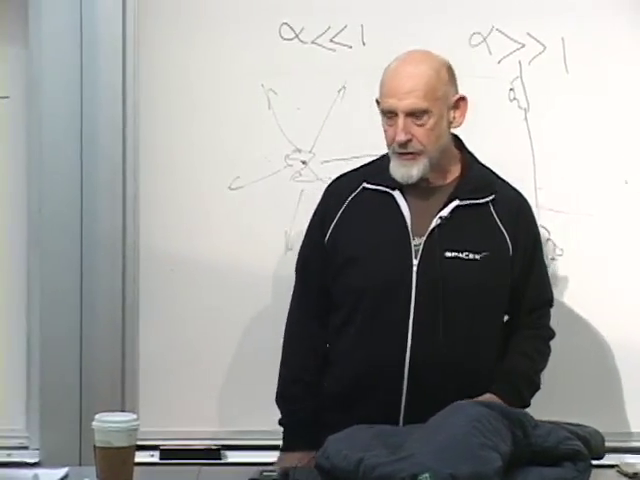
\includegraphics[width=0.72\textwidth]{lecture_01_figure_02.png}
\lectureframe{00:38:22.500}

\vspace{1em}

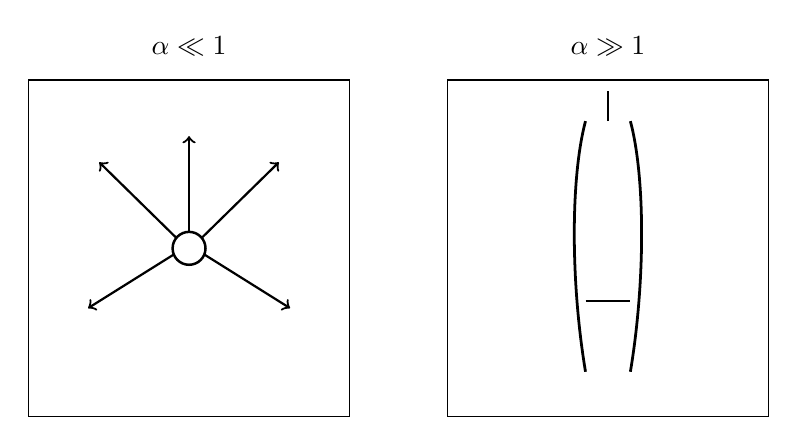
\begin{tikzpicture}[scale=0.95]
\draw (-5.3,-2.4) rectangle (-1.0,2.1);
\draw (0.3,-2.4) rectangle (4.6,2.1);

\node at (-3.15,2.55) {$\alpha \ll 1$};
\node at (2.45,2.55) {$\alpha \gg 1$};

\draw[line width=0.9pt] (-3.15,-0.15) circle (0.22);
\draw[->,line width=0.8pt] (-3.15,0.07) -- (-3.15,1.35);
\draw[->,line width=0.8pt] (-2.98,-0.01) -- (-1.95,1.00);
\draw[->,line width=0.8pt] (-3.32,-0.01) -- (-4.35,1.00);
\draw[->,line width=0.8pt] (-2.95,-0.23) -- (-1.80,-0.95);
\draw[->,line width=0.8pt] (-3.35,-0.23) -- (-4.50,-0.95);

\draw[line width=1.0pt] (2.15,-1.8) .. controls (1.95,-0.6) and (1.95,0.8) .. (2.15,1.55);
\draw[line width=1.0pt] (2.75,-1.8) .. controls (2.95,-0.6) and (2.95,0.8) .. (2.75,1.55);
\draw[line width=0.8pt] (2.15,-0.85) -- (2.75,-0.85);
\draw[line width=0.8pt] (2.45,1.55) -- (2.45,1.95);
\end{tikzpicture}\caption{Der Vergleich zwischen schwacher--starker Kopplung in der QED während der Diskussion über die Wechselwirkungsenergie. Die Abbildung stellt die beiden Regime einander gegenüber, die Susskind hier behandelt: eine dünne Wolke bei schwacher Kopplung und eine anwachsende Wolke bei starker Kopplung.}\end{figure}

Diese Abbildung gehört hierher, obwohl der Vergleich zwischen schwacher--starker Kopplung schon früher eingeführt wurde, weil Susskind den Gegensatz in der Vorlesung an dieser späteren, durch eine Frage angestoßenen Stelle bei der Diskussion der Wechselwirkungsenergie und der anwachsenden Struktur erneut zeichnet.

\section{Theorien mit geradzahligen Branen und die Entstehung einer zusätzlichen Dimension}

Bis hierher hat die Vorlesung einen deutlichen Austausch beschrieben: Fermion gegen Boson, Elektron gegen Monopol, F-String gegen D-String. Der nächste Schritt ist überraschender. Susskind wechselt zu einer anderen Variante der Stringtheorie, in der es geradzahlige statt ungeradzahlige D-Branen gibt. Dieser Unterschied ist wichtig, denn in dieser Theorie gibt es keinen D-String, der mit dem F-String ausgetauscht werden könnte. Es gibt D0-Branen, D2-Branen, D4-Branen und so weiter.

Der Grenzfall starker Kopplung kann daher nicht einfach darin bestehen, einen String durch einen anderen zu ersetzen. Laut Vorlesung geschieht etwas Seltsameres: Eine zusätzliche Raumdimension wird manifest. Susskind formuliert dies zunächst bewusst dramatisch --- ``eine neue Dimension wird sichtbar'' --- und präzisiert es unmittelbar darauf: Eine sehr kleine kompakte Richtung dehnt sich so weit aus, dass sie nicht länger vernachlässigt werden kann.

Auch die Zählung gehört zum Argument, daher hält er kurz inne:
\begin{equation}
\begin{aligned}
10\text{-dimensional string theory} &= 9\text{ space}+1\text{ time},\\
11\text{-dimensional theory} &= 10\text{ space}+1\text{ time}.
\end{aligned}
\end{equation}
Die Aussage der Vorlesung ist, dass die Theorie mit geradzahligen Branen im Grenzfall starker Kopplung effektiv elfdimensional ist.

\editorialnote{Die Theorie mit geradzahligen Branen ist die Stringtheorie vom Typ IIA; ihre Vervollständigung bei starker Kopplung ist die M-Theorie. In üblichen Einheiten skalieren der Radius des entstehenden Kreises und die elfdimensionale Planck-Länge wie folgt: \(R_{11}=g_s\ell_s\) und \(\ell_{11}=g_s^{1/3}\ell_s\). Diese Bezeichnungen und Formeln machen die moderne Zuordnung hinter der geometrischen Darstellung der Vorlesung ausdrücklich.}

\subsection{Das Erdnussbutter-Sandwich}

Um sich die kompakte Richtung vorzustellen, verwendet Susskind das Modell des ``Erdnussbutter-Sandwiches'': zwei unendlich dünne Brotscheiben mit realem Raum dazwischen. Die besondere Regel lautet, dass man auf der einen Seite hinausgeht und auf der anderen wieder hereinkommt. In einer üblichen Notation, die die Vorlesung bildlich statt formal beschreibt, kann man schreiben:
\begin{equation}
y \sim y + 2\pi R.
\end{equation}
Ist \(R\) sehr klein, beschreiben Beobachter, die im Sandwich leben, ihre Welt effektiv als niedrigdimensional. Die entscheidende Änderung bei starker Kopplung lautet dann:
\begin{equation}
g\uparrow
\qquad \Longrightarrow \qquad
R_{\mathrm{compact}}\uparrow.
\end{equation}
Wenn Susskind sagt, eine neue Raumdimension trete auf, meint er damit nicht, dass Raum aus dem Nichts entsteht. Vielmehr dehnt sich eine zuvor winzige kompakte Richtung aus und wird in der effektiven Theorie sichtbar.

\begin{figure}[htbp]\centering
\resizebox{\linewidth}{!}{%
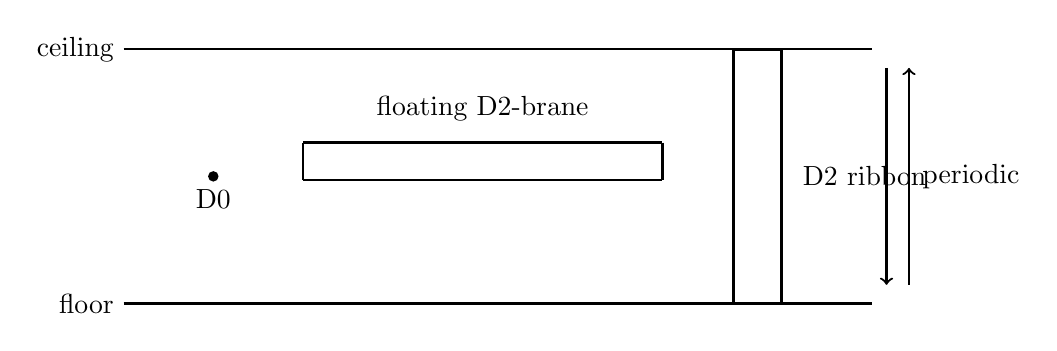
\begin{tikzpicture}[scale=0.95]
\draw[line width=0.9pt] (-5,1.7) -- (5,1.7);
\draw[line width=0.9pt] (-5,-1.7) -- (5,-1.7);

\node[left] at (-5,1.7) {ceiling};
\node[left] at (-5,-1.7) {floor};

\draw[->,line width=0.8pt] (5.2,1.45) -- (5.2,-1.45);
\draw[->,line width=0.8pt] (5.5,-1.45) -- (5.5,1.45);
\node[right] at (5.55,0) {periodic};

\draw[line width=1.0pt] (-2.6,0.45) -- (2.2,0.45);
\draw[line width=1.0pt] (-2.6,-0.05) -- (2.2,-0.05);
\draw[line width=1.0pt] (-2.6,0.45) -- (-2.6,-0.05);
\draw[line width=1.0pt] (2.2,0.45) -- (2.2,-0.05);
\node at (-0.2,0.9) {floating D2-brane};

\draw[line width=1.0pt] (3.15,-1.7) -- (3.8,-1.7);
\draw[line width=1.0pt] (3.15,1.7) -- (3.8,1.7);
\draw[line width=1.0pt] (3.15,-1.7) -- (3.15,1.7);
\draw[line width=1.0pt] (3.8,-1.7) -- (3.8,1.7);
\node[right] at (3.95,0) {D2 ribbon};

\fill (-3.8,0) circle (0.07);
\node[below] at (-3.8,-0.05) {D0};
\end{tikzpicture}}%
\caption{Die Kompaktifizierung als Sandwich. Die obere und untere Begrenzung werden periodisch miteinander identifiziert. Eine D2-Brane schwebt dazwischen wie ein Teppich, während sich eine andere vom Boden bis zur Decke erstreckt und bei kleiner kompakter Richtung wie ein String aussieht.}\end{figure}

\subsection{Was wird aus den D0- und D2-Branen?}

Nun fragt die Vorlesung, was mit den D0-Branen und den Strings geschieht. Die Antwort fällt unterschiedlich aus. Mit wachsendem \(g\) werden die D0-Branen immer leichter; in der höherdimensionalen Deutung gehören sie zum Turm der Teilchen, die Impuls in der neu sichtbaren Richtung tragen. So wird ein schweres, kompliziertes Objekt in der Beschreibung bei schwacher Kopplung zu einer gewöhnlichen leichten Anregung in der Beschreibung bei starker Kopplung.

Die Massenbeziehung zeigt die Identifikation:
\begin{equation}
M_{D0}(n)=\frac{n}{g_s\ell_s}
=\frac{n}{R_{11}}
=M_{\mathrm{KK}}(n).
\end{equation}
\editorialnote{Susskind nennt die D0-Branen ``die Gravitonen'' der elfdimensionalen Theorie. Genauer gesagt sind ihre gebundenen Zustände die Kaluza--Klein-Impulsmoden des elfdimensionalen Supergravitationsmultipletts, dessen masseloser Sektor das Graviton enthält. Diese Unterscheidung erhält die physikalische Identifikation der Vorlesung, ohne ein einzelnes Teilchen zu behaupten.}

Die D2-Branen erklären, was aus den Strings wird. Die Vorlesung hebt zwei Konfigurationen hervor:
\begin{enumerate}
\item Eine D2-Brane schwebt wie ein Teppich in der Erdnussbutter zwischen Boden und Decke.
\item Eine D2-Brane erstreckt sich wie ein Band vom Boden bis zur Decke entlang der sichtbaren Richtung.
\end{enumerate}
Ist das Sandwich dünn, erscheint das Band effektiv eindimensional. Es ist das Objekt, das Beobachter bei niedrigen Energien als String bezeichnen. Öffnet sich die kompakte Richtung, wird dasselbe Objekt eindeutig membranartig. Da es nun auch in vertikaler Richtung mehr Ausdehnung besitzt, wird es schwer und verliert seinen stringartigen Charakter.

\paragraph{Die Logik des Übergangs.}
\begin{enumerate}
\item Man beginne mit einer sehr kleinen kompakten Dimension, sodass sich das Band von Boden bis Decke effektiv wie eine Saite verhält.
\item Erhöht man \(g\), so dehnt sich die kompakte Dimension aus.
\item Die D0-Branen werden leicht und als Kaluza--Klein-Impulszustände in der höherdimensionalen Theorie neu interpretiert.
\item Das saitenartige D2-Band wird zu einer sichtbar ausgedehnten Membran und wird schwer.
\end{enumerate}
Hier liegt der Übergang der Vorlesung von der Dualität zur emergenten Geometrie. Starke Kopplung tauscht nicht bloß ein Objekt gegen ein anderes aus; sie verändert, welche Geometrie die zweckmäßigste Beschreibung ist.

Susskind hält inne und betont, wie seltsam das klingt. Das Geflecht vorgeschlagener Identifikationen erforderte schwierige mathematische Konsistenzbeziehungen. Einige davon erschienen Physikern zunächst als Vermutungen und wurden später von Mathematikern bewiesen. Er behauptet nicht, dass jedes realistische Stringvakuum verstanden sei, sondern dass das Dualitätsgeflecht selbst ungewöhnlich strengen Prüfungen standgehalten hat.

Wenn die Kopplung in diesem idealisierten Szenario von Ort zu Ort variiert, kann sich auch die zweckmäßigste Geometrie mit ihr ändern. Eine Region kann nahezu zehn-dimensional erscheinen, mit leichten Strings und schweren D0-Branen; eine andere kann sich zur elfdimensionalen Beschreibung öffnen, mit schweren gewickelten Membranen und leichten Kaluza--Klein-Moden. Der lokale Wechsel der Beschreibung ist Teil desselben Dualitätsgeflechts.

Im Transkript wird der Name dieser Beziehungen kurz als ``Ungleichungen'' wiedergegeben. Gemeint ist im Zusammenhang jedoch \emph{Dualitäten}: Beziehungen zwischen den entgegengesetzten Enden des Parameterraums. Die Korrektur ist wichtig, denn die Schlussfolgerung der Vorlesung lautet gerade, dass keine eindeutige Liste fundamentaler Bestandteile bekannt ist. Strings, Branen, Teilchen und höherdimensionale Geometrie können ineinander übergehen; entweder ist kein Element des Geflechts absolut fundamental, oder eine tiefere Ordnung ist noch unbekannt.

\section{D3-Branen, gewickelte Membranen und ein geometrisches Bild der Dualität}

Nach der Pause beschreibt Susskind das Thema ausdrücklich als ein ``riesiges Geflecht'' miteinander verbundener Theorien und Ideen. Die folgenden Beispiele sind keine neuen, isolierten Effekte, sondern Verbindungen, die die zuvor behandelten Aspekte miteinander verknüpfen.

\subsection{Eine D3-Branen-Weltvolumen}

Die erste Verbindung beruht auf einer D3-Brane. Eine D3-Brane hat drei räumliche Dimensionen, und ein auf sie beschränkter Beobachter kann sie leicht für gewöhnlichen Raum halten. Die Brane kann sich krümmen und fluktuieren, während Strings, die auf ihr enden, sich verbinden, aufspalten und streuen können. Für einen Beobachter, der nur die Richtungen entlang der Brane sieht, erscheint jeder Endpunkt als Teilchen und die Wechselwirkungen zwischen den Endpunkten wie eine gewöhnliche Quantenfeldtheorie.

\begin{figure}[htbp]
\centering
\resizebox{\linewidth}{!}{%
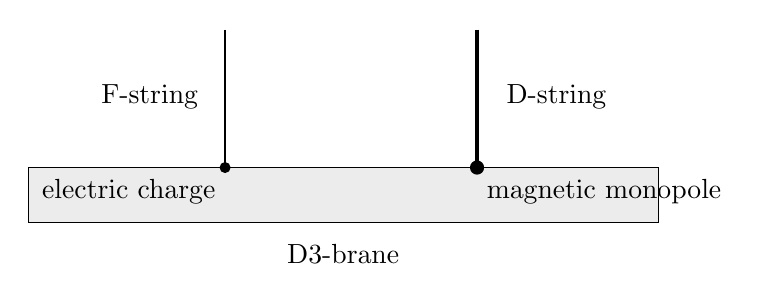
\begin{tikzpicture}[scale=1.0]
\draw[fill=gray!15] (-4,-0.35) rectangle (4,0.35);
\node at (0,-0.75) {D3-brane};

\draw[line width=0.9pt] (-1.5,2.1) -- (-1.5,0.35);
\fill (-1.5,0.35) circle (0.07);
\node[left] at (-1.72,1.25) {F-string};
\node[below left] at (-1.5,0.32) {electric charge};

\draw[line width=1.5pt] (1.7,2.1) -- (1.7,0.35);
\fill (1.7,0.35) circle (0.09);
\node[right] at (1.95,1.25) {D-string};
\node[below right] at (1.7,0.32) {magnetic monopole};
\end{tikzpicture}
}%
\caption{Deutung über das Weltvolumen der D3-Brane. Der Endpunkt eines F-Strings erscheint als elektrische Ladung; der Endpunkt eines D-Strings als magnetischer Monopol.}
\end{figure}

Dies ist eine der überzeugendsten Identifikationen der Vorlesung. Für einen Beobachter auf dem Weltvolumen erscheint ein auf der D3-Brane endender F-String als elektrische Ladung. Ein auf derselben Brane endender D-String erscheint als magnetischer Monopol. Anders gesagt: Die Dualität zwischen F-Strings und D-Strings wird auf dem Weltvolumen der D3-Brane zur elektrisch--magnetischen Dualität der gewöhnlichen Feldtheorie. Was zuvor eine Analogie war, ist nun eine explizite Zuordnung.

\editorialnote{Für einen Stapel von D3-Branen ist die niederenergetische Beschreibung auf dem Weltvolumen eine vierdimensionale \(\mathcal N=4\) supersymmetrische Yang--Mills-Theorie. Ihre elektrisch--magnetische Dualität ist die feldtheoretische Realisierung der S-Dualität der Typ-IIB-Theorie; eine einzelne Brane liefert den in der Vorlesung bildlich dargestellten abelschen Grenzfall.}

\subsection{Zwei kompakte Dimensionen und asymmetrische Wicklung}

Anschließend kehrt Susskind zur höherdimensionalen Geometrie zurück und kompaktifiziert nicht eine, sondern zwei kleine Dimensionen. Da sich elf Dimensionen nicht an eine Tafel zeichnen lassen, fasst er die sieben großen, in der Skizze nicht verwendeten Dimensionen zu einer sichtbaren horizontalen Richtung zusammen und zeichnet die beiden kompakten Dimensionen ausdrücklich ein. Er besteht auf einer asymmetrischen Darstellung der Kompaktifizierung, denn eine kompakte Richtung muss kürzer sein als die andere, wenn die effektiven Strings unterschiedliche Spannungen haben sollen.

\begin{figure}[htbp]
\centering
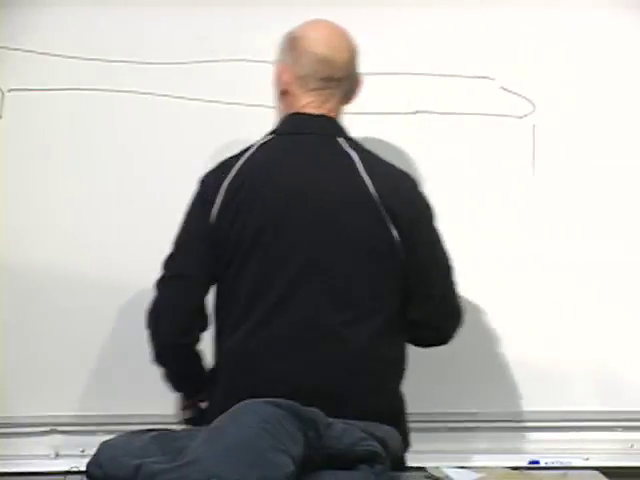
\includegraphics[width=0.78\textwidth]{lecture_01_figure_03.png}
\lectureframe{01:10:25.000}
\caption{Der fertige Tafelstand mit den beiden gewickelten Membranen. Die kurzen und langen kompakten Zyklen ergeben die rechts gezeichneten F- und D-stringartigen Bänder.}
\end{figure}

Eine Membran kann um eine der beiden kompakten Richtungen gewickelt sein und aus Sicht der nichtkompakten Richtungen wie ein String aussehen. Sind \(R_1\) und \(R_2\) die Radien der beiden Kreise, so lauten die effektiven Spannungen
\begin{equation}
\begin{aligned}
T_{(1)}&=2\pi R_1 T_{\mathrm{M2}},\\
T_{(2)}&=2\pi R_2 T_{\mathrm{M2}},\\
\frac{T_{(1)}}{T_{(2)}}&=\frac{R_1}{R_2}.
\end{aligned}
\end{equation}
Unterschiedliche Kreisgrößen führen also zu unterschiedlichen Stringspannungen. Identifiziert man die Wicklung um den kürzeren Kreis mit dem leichten F-String und die um den längeren mit dem schweren D-String, kann man schematisch schreiben:
\begin{equation}
g_s\sim \frac{R_{\mathrm{short}}}{R_{\mathrm{long}}},
\qquad
\frac{T_{\mathrm{D1}}}{T_{\mathrm{F1}}}\sim \frac{1}{g_s}.
\end{equation}

\begin{classroomqa}
\audiencequestion{Lässt sich die Kopplung in diesem Bild als Verhältnis der beiden kompakten Dimensionen verstehen? \lecturetimestamp{01:10:13}}
\lecturerresponse{Ja. Der Parameter für schwache--starke Kopplung wird geometrisch als Seitenverhältnis dargestellt. Wird eine Richtung verkürzt, ergibt sich eine kleine Kopplung; beim Vertauschen der beiden Richtungen werden die leichten und schweren Strings vertauscht.}
\end{classroomqa}

\editorialnote{In der Vorlesung wird dieses Verhältnis vorübergehend mit \(\alpha\) bezeichnet, wobei dasselbe Symbol wie zuvor für die Feinstrukturkonstante der QED verwendet wird. Hier schreiben wir \(g_s\), um die beiden Bedeutungen auseinanderzuhalten. In der vollständigen M-Theorie-Konstruktion ist die Kopplung der Typ-IIB-Theorie in der komplexen Struktur des kompakten Zweitorus kodiert; welcher Ausdruck genau im Zähler steht, hängt davon ab, wie seine Zyklen bezeichnet werden.}

Das Bild der gewickelten Membran lässt sich ohne die perspektivische Verzerrung der Tafelzeichnung so zusammenfassen:

\begin{figure}[htbp]
\centering
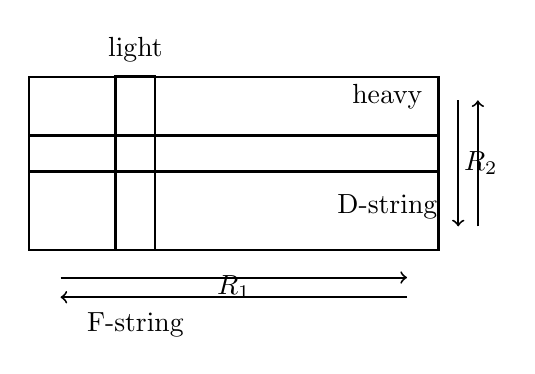
\begin{tikzpicture}[scale=1.0]
\draw[line width=0.9pt] (0,0) rectangle (5.2,2.2);
\node[below] at (2.6,-0.2) {\(R_1\)};
\node[right] at (5.4,1.1) {\(R_2\)};

\draw[->,line width=0.7pt] (5.45,1.9) -- (5.45,0.3);
\draw[->,line width=0.7pt] (5.7,0.3) -- (5.7,1.9);
\draw[->,line width=0.7pt] (0.4,-0.35) -- (4.8,-0.35);
\draw[->,line width=0.7pt] (4.8,-0.6) -- (0.4,-0.6);

\draw[line width=1.0pt] (1.1,0) -- (1.6,0) -- (1.6,2.2) -- (1.1,2.2) -- cycle;
\node at (1.35,2.55) {light};

\draw[line width=1.0pt] (0,1.45) -- (5.2,1.45);
\draw[line width=1.0pt] (0,1.00) -- (5.2,1.00);
\node at (4.55,1.95) {heavy};

\node at (1.35,-0.95) {F-string};
\node at (4.55,0.55) {D-string};
\end{tikzpicture}
\caption{Zwei gewickelte Membrankonfigurationen erscheinen aus Sicht der nichtkompakten Richtungen beide als Strings. Unterschiedliche kompakte Skalen sorgen jedoch dafür, dass einer der effektiven Strings leichter ist als der andere.}
\end{figure}

Dies ist die geometrische Version der zuvor erläuterten Dualität. Drückt man eine Richtung zusammen und dehnt die andere, wird das eine gewickelte Objekt schwerer und das andere leichter; so können F-String und D-String ihre Rollen tauschen.

\begin{classroomqa}
\audiencequestion{Sind die kompakten Richtungen zyklisch, sind die gewickelten Objekte dann unendlich breit? \lecturetimestamp{01:10:41}}
\lecturerresponse{Nein. Ein kompakter Kreis hat einen endlichen Umfang, obwohl man ihn wiederholt durchlaufen kann, ohne je einen Rand zu erreichen. Ober- und Unterkante der aufgeschnittenen Zeichnung stellen denselben Punkt dar, so wie die Endpunkte eines Intervalls denselben Punkt auf einem Kreis darstellen können.}
\end{classroomqa}

\begin{figure}[htbp]
\centering
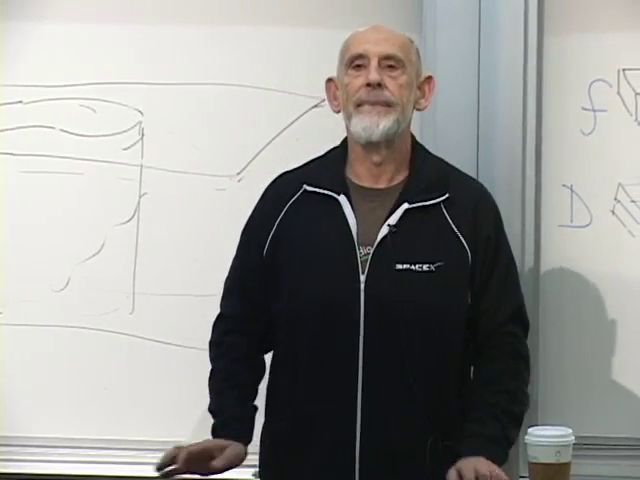
\includegraphics[width=0.78\textwidth]{lecture_01_figure_04.png}
\lectureframe{01:12:25.000}

\vspace{1em}

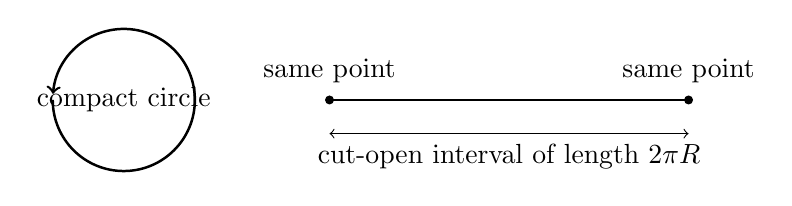
\begin{tikzpicture}[scale=0.95]
\draw[line width=0.9pt,->] (-3.7,0) arc[start angle=180,end angle=535,radius=0.95];
\node at (-2.75,0) {compact circle};
\draw[line width=0.9pt] (0.0,0) -- (4.8,0);
\fill (0.0,0) circle (0.06);
\fill (4.8,0) circle (0.06);
\draw[<->] (0.0,-0.45) -- (4.8,-0.45);
\node at (2.4,-0.75) {cut-open interval of length \(2\pi R\)};
\node[above] at (0.0,0.1) {same point};
\node[above] at (4.8,0.1) {same point};
\end{tikzpicture}
\caption{Ein kompakter Kreis und seine aufgeschnittene Darstellung an der Tafel. Überschreitet man den einen Endpunkt, gelangt man am anderen wieder hinein; bewegt man sich zugleich in einer nichtkompakten Richtung um den Kreis, beschreibt man dagegen eine Schraubenlinie.}
\end{figure}

\begin{classroomqa}
\audiencequestion{Warum ist der kompakte Weg ein Kreis und keine Schraubenlinie? \lecturetimestamp{01:12:23}}
\lecturerresponse{An jedem festen Punkt in der nichtkompakten Richtung ist die kompakte Richtung ein Kreis. Eine Schraubenlinie entsteht nur, wenn man sich in der nichtkompakten Richtung weiterbewegt und zugleich den Kreis umläuft. Das an der Tafel gezeichnete Intervall ist einfach ein aufgeschnittener Kreis, dessen beiden Endpunkte miteinander identifiziert werden.}
\end{classroomqa}

\begin{classroomqa}
\audiencequestion{Erklärt diese Geometrie selbst, wie eine D-Brane bei genauer Untersuchung wie eine Ansammlung von F-Strings aussehen kann? \lecturetimestamp{01:12:49}}
\lecturerresponse{Der Zusammenhang ist vorhanden, aber in diesem einfachen Bild nicht unmittelbar ersichtlich; um ihn zu erkennen, braucht es weitergehende geometrische Mittel. Die Skizze soll die Dualität ordnen, nicht jede mikroskopische Beschreibung der Bestandteile herleiten.}
\end{classroomqa}

\begin{classroomqa}
\audiencequestion{Können sich die langen und kurzen kompakten Richtungen beim Durchlaufen des Raums oder im Lauf der Zeit vertauschen? \lecturetimestamp{01:13:35}}
\lecturerresponse{Im idealisierten Modell ist beides möglich. Wird ein Zyklus gestaucht und der andere gedehnt, vertauscht sich, welcher gewickelte String leicht ist. Das ist ein weiterer Grund dafür, dass ``fundamentaler String'' nur eine Bezeichnung ist: Die zweckmäßigste Beschreibung kann sich von einer Region zur anderen oder mit der Zeit ändern.}
\end{classroomqa}

\section{Idealisierung, besonders symmetrische Punkte und die Landschaft}

Im letzten Teil der Vorlesung tritt Susskind von den eleganten Dualitätsbeispielen zurück und fragt, was sie uns über die reale Welt sagen und was nicht.

Zunächst warnt Susskind, dass die präzise kontrollierbaren Dualitäten Eigenschaften stark idealisierter supersymmetrischer Theorien sind, in denen Bosonen und Fermionen exakt übereinstimmende Massen haben. Als Analogie nennt er Kreisbahnen in der Newtonschen Mechanik: Man untersucht sie zuerst, weil sie symmetrisch und mathematisch handhabbar sind, nicht weil sich die tatsächliche Planetenbewegung auf perfekte Kreise beschränkt. Genauso lassen sich supersymmetrische Stringtheorien leichter analysieren, weil sie symmetrischer sind als die Natur zu sein scheint.

Die Idealisierung ist dennoch aufschlussreich. Eine perfekte Kreisbahn ist kein realistisches Planetensystem, zeigt aber Eigenschaften, die auch bei weniger symmetrischen Bahnen erhalten bleiben. Ebenso zeigen die supersymmetrischen Beispiele konsistente Möglichkeiten, Quantenmechanik, Gravitation und mikroskopische Struktur miteinander zu vereinbaren. Susskind formuliert bewusst zugespitzt: Die handhabbaren Stringtheorien sind buchstäblich nicht die Theorie unserer Welt; ihr Wert liegt darin, dass sie Phänomene offenbaren, die wahrscheinlich auch in weniger symmetrischen und weniger handhabbaren Situationen wieder auftreten.

\subsection{Ein Baukasten mit vielen möglichen Ergebnissen}

D-Branen sind nur ein Teil des verfügbaren Baukastens. Die Vorlesung nennt auch Flüsse, Orbifolds und Orientifolds. Zunächst wählt man eine kompakte Geometrie und dann, welche Branen und Flüsse ihre Zyklen besetzen. Selbst beim einfachen Sandwich ändert sich die niederdimensionale Physik, wenn man eine schwebende D2-Brane, zwei oder drei einfügt. Fügt man solche Bestandteile hinzu oder entfernt sie, ändern sich die effektiven Teilchen, Wechselwirkungen und Parameter.

Angenommen, ein sechsdimensionaler kompakter Raum habe in der schematischen Zählung der Vorlesung etwa \(500\) Zyklen, und für jeden Zyklus gebe es ungefähr \(10\) Möglichkeiten, gewickelte Branen, Flüsse oder verwandte Strukturen zu wählen. Dann wächst die Zahl der Konstruktionen wie
\begin{equation}
N_{\mathrm{vacua}} \sim 10^{500}.
\end{equation}
Die Zähllogik der Vorlesung ist einfach:
\begin{equation}
10 \times 10 \times \cdots \times 10 = 10^{500}
\end{equation}
mit \(500\) Faktoren. Die Analogie mit der DNA verdeutlicht denselben Punkt auf vertrautere Weise:
\begin{equation}
N_{\mathrm{DNA}}(500)=4^{500}.
\end{equation}
Während des DNA-Vergleichs fragt ein Zuhörer nach und vergewissert sich, dass es entlang eines Strangs vier Alternativen gibt: A, C, G und T. Die Korrektur verstärkt das Argument, statt es zu verändern. Eine kurze Liste lokaler Möglichkeiten, viele Male wiederholt, ergibt eine riesige Zahl globaler Anordnungen. Der genaue Exponent ist nicht entscheidend, und Susskind bezeichnet \(10^{500}\) als alte Unterschätzung; entscheidend ist die kombinatorische Vervielfachung.

Damit kehrt sich die reduktionistische Erwartung vom Anfang der Vorlesung endgültig um. Eine komplizierte Teilchenphysik muss nicht aus komplizierten mikroskopischen Regeln hervorgehen. Sie kann entstehen, weil unser Vakuum eine komplizierte Anordnung vieler einfacher Bestandteile ist, so wie ein komplexer Organismus durch eine Sequenz kodiert sein kann, die aus vier Basen aufgebaut ist.

\begin{classroomqa}
\audiencequestion{Würde vollständige Kenntnis nach der Identifizierung dualitätsverwandter äquivalenter Beschreibungen nur ein oder wenige dieser möglichen Vakua als Beschreibungen unserer Welt auswählen? \lecturetimestamp{01:26:11}}
\lecturerresponse{Vermutlich würde sie eine eingeschränkte Menge auswählen, doch viele verschiedene Vakua könnten bei zugänglichen Energien äußerst ähnlich aussehen. Die zitierte Anzahl möglicher Vakua soll auch nach der Identifizierung dualer Beschreibungen groß bleiben, und irrelevante Details bei hohen Energien können wie ``„Junk-DNA“''} wirken.\end{classroomqa}

\subsection{Symmetrische Punkte und generische Komplexität}

In der Landschaft gibt es besonders symmetrische Punkte. Im geometrischen Bild macht eine Konfiguration mit gleichen Seitenverhältnissen,
\begin{equation}
R_1=R_2,
\end{equation}
die beiden gewickelten Beschreibungen gleichermaßen einfach. In der Analogie mit elektrisch--magnetischer Dualität wird dies schematisch dargestellt durch
\begin{equation}
m_{\mathrm{monopole}}=m_e.
\end{equation}

\begin{figure}[htbp]
\centering
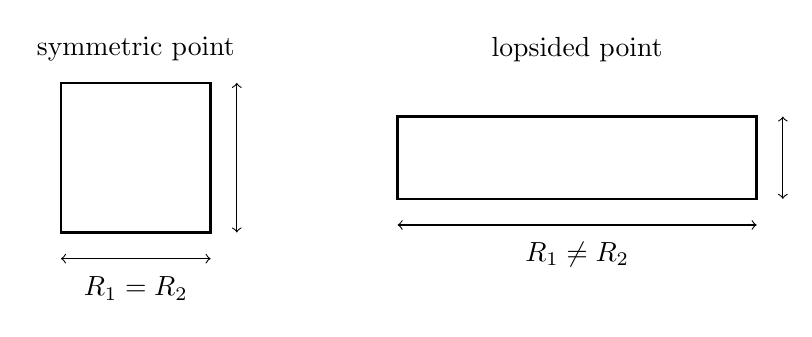
\begin{tikzpicture}[scale=0.95]
\draw[line width=0.9pt] (-4.5,-1.0) rectangle (-2.5,1.0);
\draw[<->] (-4.5,-1.35) -- (-2.5,-1.35);
\draw[<->] (-2.15,-1.0) -- (-2.15,1.0);
\node at (-3.5,1.45) {symmetric point};
\node at (-3.5,-1.75) {$R_1=R_2$};

\draw[line width=0.9pt] (0.0,-0.55) rectangle (4.8,0.55);
\draw[<->] (0.0,-0.9) -- (4.8,-0.9);
\draw[<->] (5.15,-0.55) -- (5.15,0.55);
\node at (2.4,1.45) {lopsided point};
\node at (2.4,-1.3) {$R_1\ne R_2$};
\end{tikzpicture}
\caption{Eine Kompaktifizierung mit gleichen Seitenverhältnissen behandelt die beiden gewickelten Strings symmetrisch; bei einer stark verzerrten Kompaktifizierung ist eine der Beschreibungen deutlich leichter als die andere.}
\end{figure}

\begin{classroomqa}
\audiencequestion{Gibt es in der Landschaft Vakua, bei denen die Konstruktion viel einfacher wird, weil die Beschreibungen durch F- und D-Strings zusammenfallen? \lecturetimestamp{01:27:21}}
\lecturerresponse{Ja, es gibt besonders symmetrische Punkte. Unsere Welt scheint sich nicht an einem solchen Punkt zu befinden: Das vertraute elektrische Teilchen und ein magnetischer Monopol haben nicht dieselbe Masse. Warum die Natur einen verzerrten Punkt einnimmt, ist unbekannt.}
\end{classroomqa}

\editorialnote{Die Gleichheit der Elektronen--- und Monopolmasse ist ein schematisches Merkmal eines geeignet geschützten selbstdualen Modells, keine Vorhersage der gewöhnlichen, nichtsupersymmetrischen QED. Sie bringt die Idee des symmetrischen Punkts aus der Vorlesung zum Ausdruck und ist keine Behauptung über das beobachtete Elektron.}

Anschließend erinnert Susskind an eine Analogie aus der Kommunikationstheorie. Zufällige Codes können außerordentlich gut sein, während die am einfachsten zu beschreibenden und zu dekodierenden Codes zusätzliche mathematische Struktur haben und sich historisch weniger gut bewährten. Später fand die Codierungstheorie hochwirksame strukturierte Konstruktionen, doch die Analogie bleibt bestehen: Alles, was sich knapp benennen oder beschreiben lässt, liegt in einer besonders speziellen, niedrigkomplexen Ecke des gesamten Möglichkeitsraums. Ebenso können die am leichtesten berechenbaren Stringvakua untypisch einfach sein.

Daher könnten sich die passenden Fragen ändern. Statt die genaue Kompaktifizierung bis ins mikroskopische Detail zu verlangen, kann man fragen, welche Merkmale in einem breiten Ensemble häufig oder generisch sind. Susskind stellt dies als Forschungsproblem dar, nicht als gesicherte Schlussfolgerung, und lehnt ideologische Argumente anstelle von Berechnungen ab.

\subsection{Kosmologische Fragen}

\begin{classroomqa}
\audiencequestion{Unterscheidet sich eine kompakte Richtung mit enormem Umfang bei Beobachtungen von einer unendlichen Richtung, und wissen wir, dass unsere drei großen Raumdimensionen unendlich sind? \lecturetimestamp{01:30:03}}
\lecturerresponse{Wir wissen nicht, ob sie unendlich sind. Eine geschlossene Dreisphäre kann sich ausdehnen und dabei kompakt bleiben. Messungen der nahezu flachen Geometrie liefern lediglich eine untere Schranke für den Krümmungsradius, so wie eine Vermessung eines nahezu ebenen Feldes die Größe der Erde eingrenzen kann, ohne zu beweisen, dass ihre Oberfläche unendlich ist. Erst eine nachgewiesene Krümmung oder globale Identifikation würde die endliche Skala bestimmen.}
\end{classroomqa}

\begin{classroomqa}
\audiencequestion{Wenn die Kopplung im idealisierten Modell räumlich variieren kann, wie könnte eine solche Variation in der realen Welt auftreten? \lecturetimestamp{01:32:43}}
\lecturerresponse{Nicht als die uneingeschränkte, glatte Variation im symmetrischen Beispiel. Die realistische Möglichkeit, die später behandelt wird, ist eine Variation durch diskrete Übergänge zwischen Regionen mit unterschiedlichen effektiven Gesetzen. Ob solche Sprünge auftreten, ist eine kosmologische Frage.}
\end{classroomqa}

\editorialnote{Diese Antwort ist als Vorausblick der Vorlesung auf Flussvakua und Übergänge zwischen Domänen zu verstehen, nicht als allgemeiner Satz, der jedes glatt variierende Skalarfeld ausschließt. Beobachtungen setzen Variationen dimensionsloser Kopplungen enge Grenzen; Stabilisierungsmechanismen bestimmen, ob in einem bestimmten Modell kontinuierliche Moduli verfügbar bleiben.}

Die Aufnahme enthält die letzte Frage aus dem Publikum nicht. Aus der erhaltenen Antwort geht hervor, dass das vorgeschlagene Phänomen bei bestimmten Arten von Schwarzen Löchern auftreten kann, nicht jedoch am Horizont eines gewöhnlichen Schwarzschild-Schwarzen-Lochs, dessen Horizont für einen frei fallenden Beobachter lokal ein gewöhnlicher Ort ist. Da sich die Frage nicht zuverlässig rekonstruieren lässt, wird dem Wortwechsel keine spezifischere Aussage zugeschrieben.

\section{Von Bausteinen zu einem Geflecht von Beschreibungen}

Die Hoffnung, dass tiefere Schichten der Physik einfacher sein müssen, hat sich als trügerisch erwiesen. Bei der \(1+1\)-dimensionalen Bosonisierung kann dieselbe Theorie entweder in Begriffen von Fermionen oder von Bosonen formuliert werden, wobei das Fermion als Kink wieder auftritt. In der Quantenelektrodynamik tauschen schwache und starke Kopplung die beschreibenden Rollen von Elektron und magnetischem Monopol aus. In der Stringtheorie wiederholen F-Strings und D-Strings dasselbe Muster. In der Theorie geradzahliger Branen geht die starke Kopplung noch weiter: Eine kompakte Richtung dehnt sich aus, D0-Branen werden zu Kaluza--Klein-Impulszuständen, und effektive Strings werden als gewickelte Membranen in einer höherdimensionalen Geometrie neu interpretiert. Die moderne Quantenfeldtheorie und Stringtheorie liefern daher keine einzigartige, ein für alle Mal feststehende Antwort auf die Frage ``Was sind die Bausteine und was die Häuser?'' Sie liefern ein Geflecht von Beschreibungen, deren jede in ihrem eigenen Bereich zweckmäßig ist, sowie eine riesige Landschaft möglicher Konstruktionen, deren generisches Ergebnis Komplexität statt Einfachheit ist.
